\documentclass[usenames,dvipsnames]{beamer}
\mode<presentation>{}
\usetheme{ULB}


\newcounter{FootlineChoice}
\newcounter{DepartmentLogo}
\newcounter{FacultyLogo}

\def\DepartmentLogo{theme/logos/urlab.pdf}
% In the folder "theme/logos/" please import the Department logo image. This will appear at north east corner of every frame

\setcounter{DepartmentLogo}{2}
% Please select 0 if you want a blank NE corner for each frame
% Please select 1 if you want the Department Logo only on the Title Page (NE corner)
% Please select 2 if you want the Department Logo on each frame (still NE corner)


\def\FacultyLogo{theme/logos/ulb_sciences.png}
% In the folder "theme/logos/" please import the Faculty logo image. This will appear at south east corner of title frame

\setcounter{FacultyLogo}{1}
% Please select 1 if you want the Faculty Logo to be displayed in the sE corner of the title frame
% Please select 0 if you want a blank SE corner for the title frame


%%%%%%%%%%%%%%%%%%%%%%%%%%%%%%%%%%%%%%%%%%%%%%%%% FOOTLINE MANAGEMENT %%%%%%%%%%%%%%%%%%%%%%%%%%%%%%%%%%%%%%%%%%%%%%%%%

\setcounter{FootlineChoice}{3}
% Please select value 0,1, or 2 for the footline alignment.
% All footlines display the [author] in SW corner and [institute] in SE corner,
% but you can choose between the following options for the center of the footline :

% Footline Aligment 0 : 
%       Only the current section is displayed. All is aligned with the very bottom of the frame.

% Footline Aligment 1 :
%       Only the current section is displayed. All is aligned a bit higher to escape potential crops when projecting.

% Footline Aligment 2 : 
%       Current section and subsection are displayed.  All is aligned a bit higher to escape potential crops when projecting.

% Footline Alignment 3 :
%       Nothing displayed at center. [author] and [institute] aligned with very bottom of frame.

\usepackage{xcolor}
\usepackage{caption}
\usepackage{subcaption}
\usepackage{multimedia}
\usepackage{soul}
\usepackage{svg}
\usepackage{listings}
\usepackage{inconsolata}

%add support for unicode \ding{55} and \ding{51}
\usepackage{pifont}
\newcommand{\greenv}{\textcolor{ForestGreen}{\ding{51}}}
\newcommand{\redx}{\textcolor{red}{\ding{55}}}
\newcommand{\backupbegin}{
	\newcounter{finalframe}
	\setcounter{finalframe}{\value{framenumber}}
}
\newcommand{\backupend}{
	\setcounter{framenumber}{\value{finalframe}}
}


\title{Git 101:\\ Tout ce qu'il faut connaitre pour etre un bon dev.}
\subtitle{Atelier Git(hub)}
\date{\today}
\author{Kevin \textsc{Vandervaeren}}
\institute{ULB -- URLAB}


\begin{document}

\begin{frame}[plain,noframenumbering]
	\titlepage
\end{frame}

\begin{frame}{Agenda}
	\begin{columns}
		\begin{column}{0.65\linewidth}
			\begin{itemize}
				\item<1-> donné et partage de fichiers 
				\item<2-> Introduction à Git
				\begin{itemize}
					\item comment ça marche ?
					\item quel sont les avantages ?
					\item comment l'installer ?
					\item comment l'utiliser ?
					\item exercices pratiques
				\end{itemize}
				\item<3-> Introduction à GitHub (ou autre plateforme)
				\begin{itemize}
					\item En quoi est-ce différent de Git ?
					\item Comment l'utiliser ?
					\item avantages et inconvénients
					\item exercices pratiques
				\end{itemize}
				\item<4-> Conclusion et synthèse
				\item<5-> Et pour aller plus loin
			\end{itemize}
		\end{column} %%
		\begin{column}{0.3\linewidth}
			
\includegraphics[width=\linewidth]{Im/Git-logo.png}
		\end{column}
	\end{columns}
\end{frame}

\begin{frame}[fragile]{donné et partage de fichiers}
	comment partagée des fichiers (code) entre plusieurs personnes ou plusieurs machines ?
\end{frame}

% when itemize in the next slide every item will be transparant after the previous one
\begin{frame}[fragile]{donné et partage de fichiers}
	% this slide is a bit of a joke, where I ask the audience how they store their files, and then I show them the "worst" way to do it
	% it will be presented as consecutive images on top of each other this will be showed one by one
	\begin{columns}
		\begin{column}{0.5\linewidth}
			\begin{itemize}
				\item<1-> photo de l'écran
				% create a "advantages" and "disadvantages" list
				\item<2-> une clé USB
				\item<3-> fichier sur discord
				\item<4-> Cloud (google drive, dropbox, \dots)
			\end{itemize}
		\end{column}
		\begin{column}{0.5\linewidth}
			\begin{overprint}
				\onslide<1>
\includegraphics[width=\linewidth]{Im/taking_picture_sreen.jpeg}
				\onslide<2>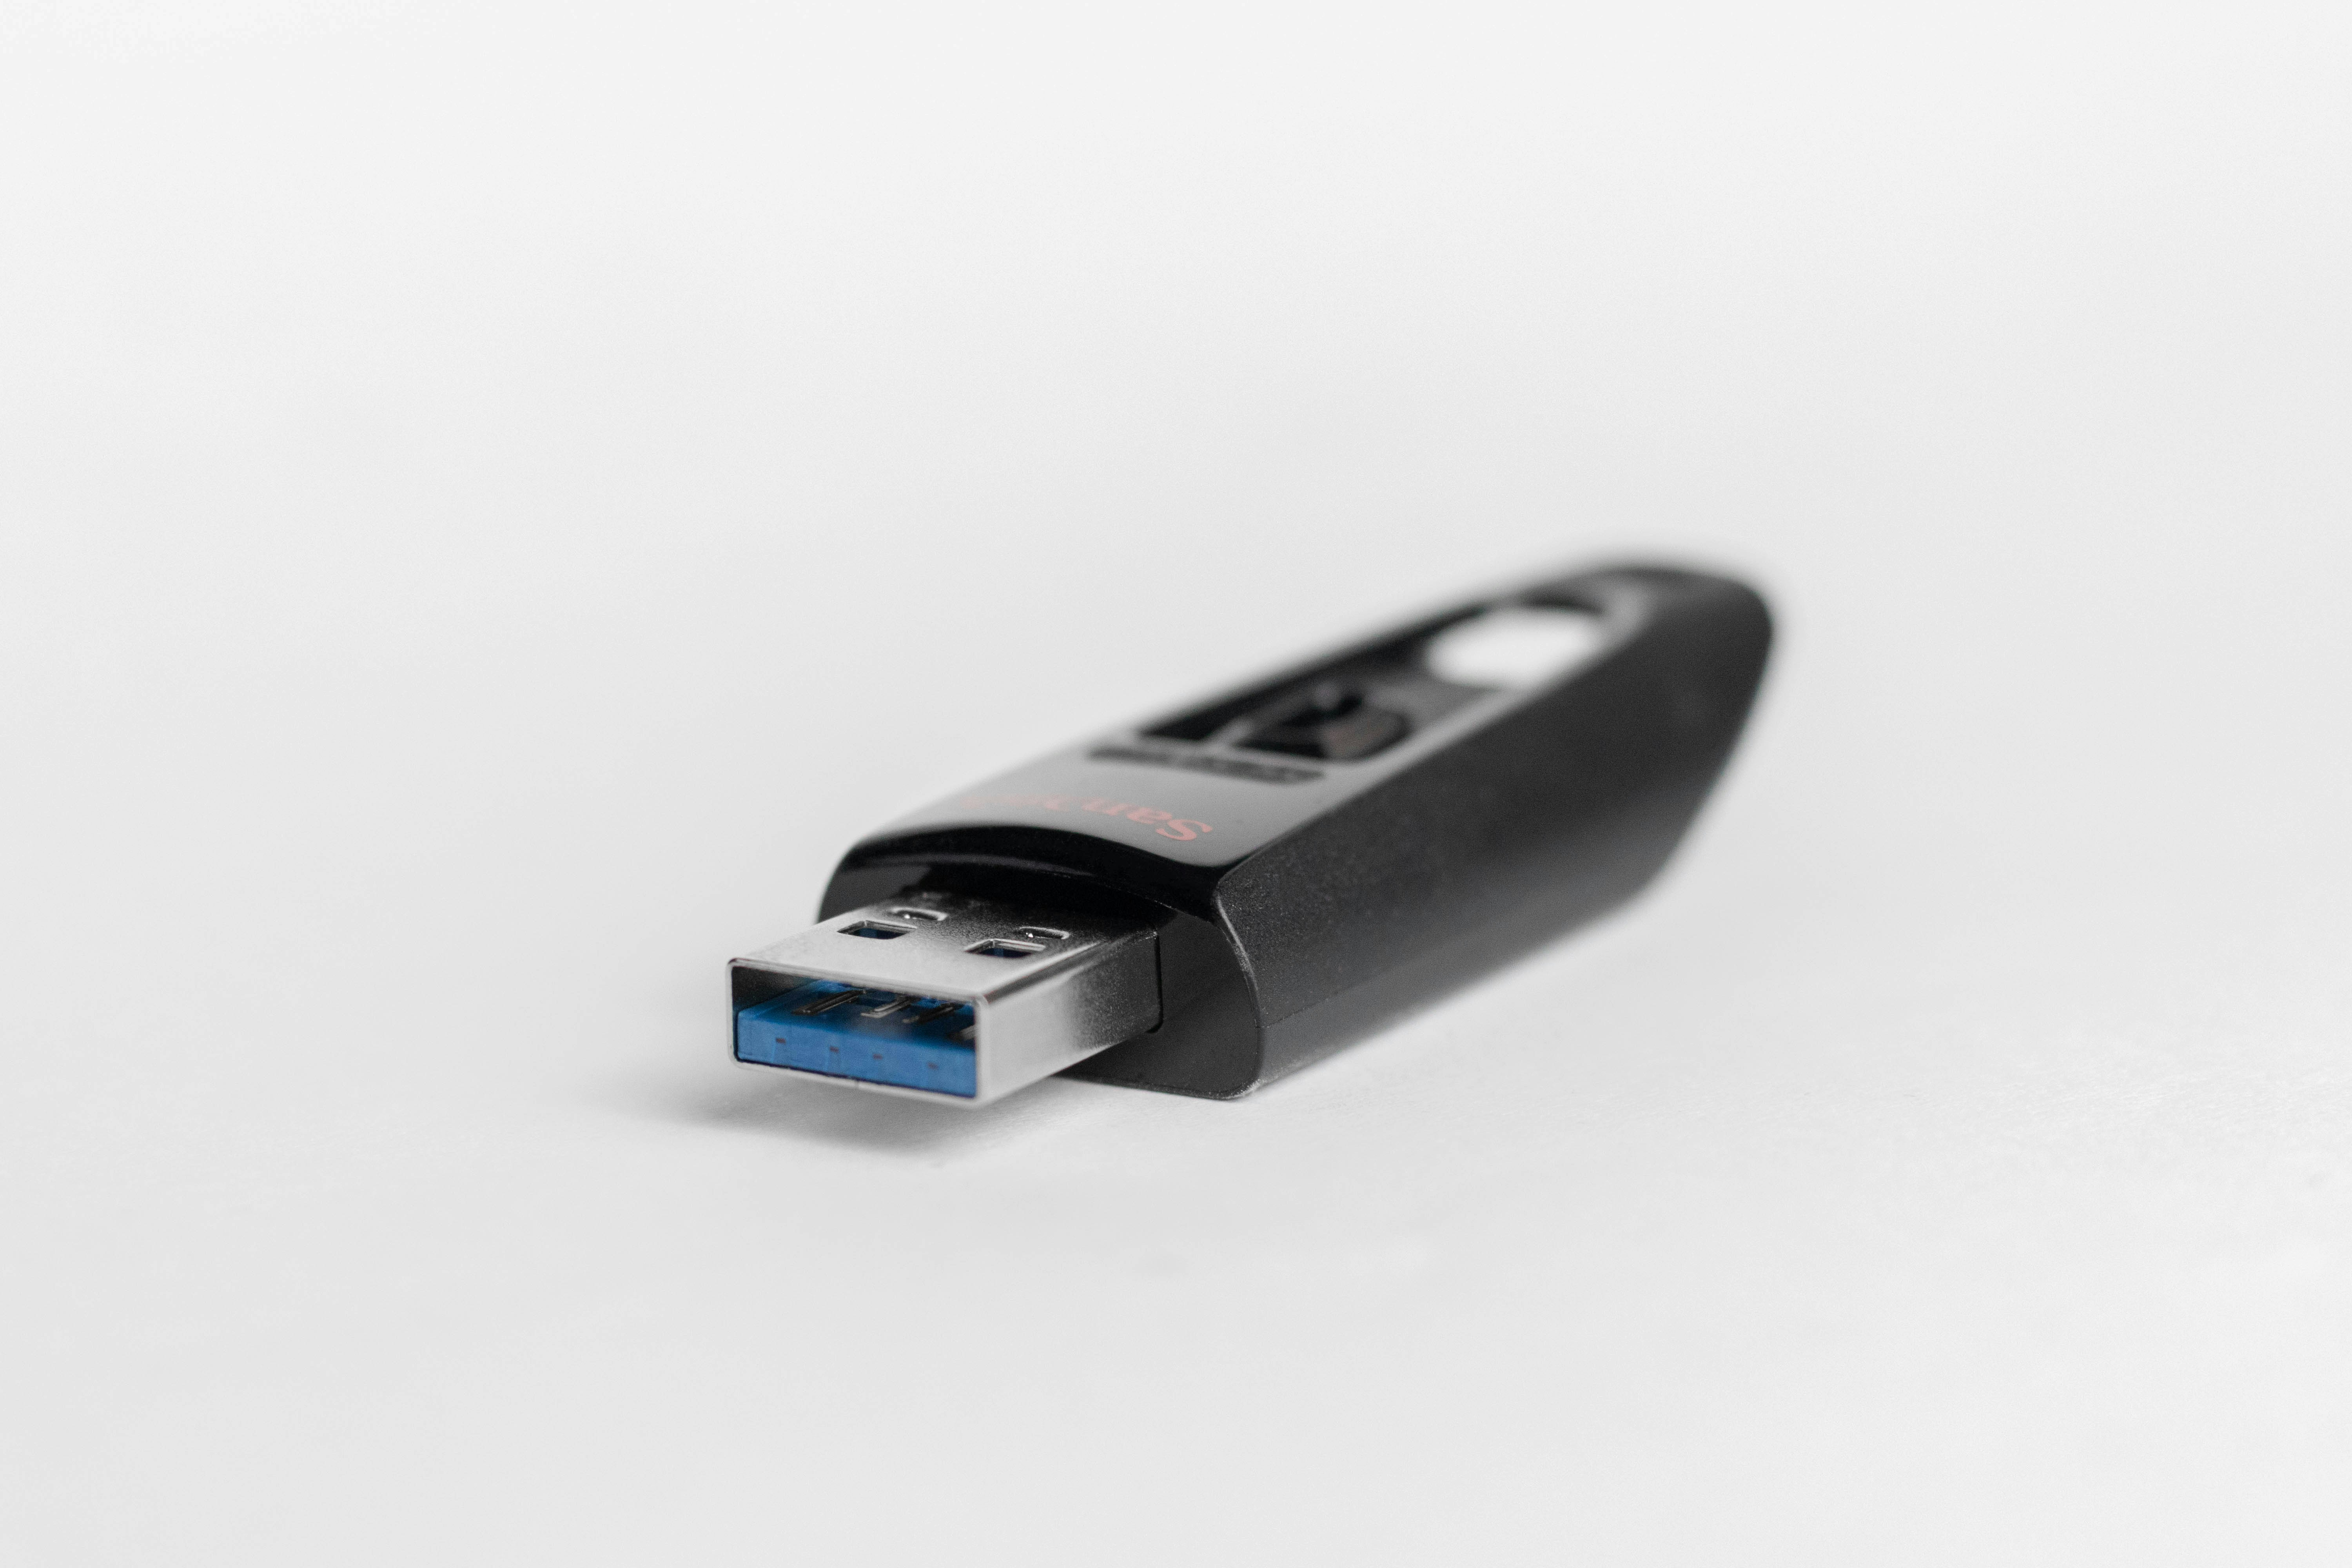
\includegraphics[width=\linewidth]{Im/thumb_drive.jpg}
				\onslide<3>
\includegraphics[width=\linewidth]{Im/discord.png}
				\onslide<4>
\includegraphics[width=\linewidth]{Im/cumulus.jpg}
			\end{overprint}
		\end{column}
	\end{columns}
\end{frame}

% add on the previous slide a small note telling that not all methods are equal
\begin{frame}[fragile]{donné et partage de fichiers}
	\begin{itemize}
		\item photo de l'écran
		\item une clé USB
		\item fichier sur discord
		\item Cloud (google drive, dropbox, \dots)
	\end{itemize}
	% add a note that not all methods are equal
	\begin{alertblock}{Attention}
		Toutes les méthodes ne se valent pas !
	\end{alertblock}
\end{frame}

\begin{frame}[fragile]{donné et partage de fichiers}
	%create a comand for the red ding{55} and green checkmark
	\resizebox{\linewidth}{!}{
		\begin{tabular}{|l|c|c|c|c|c|c|}
			\hline
			\textbf{Méthode} & \textbf{Historique} & \textbf{Sauvegarde} & \textbf{Collaboration} & \textbf{Travail en parallèle} & \textbf{Commentaires} & \textbf{Automatisation} \\ \hline
			\hline
			\textbf{Prendre une photo} & \redx & \redx & \redx & \redx & \redx & \redx \\ \hline
			\textbf{Clé USB} & \redx & \greenv & \redx & \redx & \redx & \redx \\ \hline
			\textbf{Serveur Discord} & \redx & \greenv & \greenv & \redx & \redx & \redx \\ \hline

			\textbf{Cloud} & \greenv & \greenv & \greenv & \redx & \greenv & \redx \\ \hline
		\end{tabular}
	}
\end{frame}

% now we will show the advantages and disadvantages of each of the methods using tables each line will be a method and the columns will a thing to do and the cell will be a cross or a checkmark
\begin{frame}[fragile]{donné et partage de fichiers}
	%create a comand for the red ding{55} and green checkmark
	\resizebox{\linewidth}{!}{
		\begin{tabular}{|l|c|c|c|c|c|c|}
			\hline
			\textbf{Méthode} & \textbf{Historique} & \textbf{Sauvegarde} & \textbf{Collaboration} & \textbf{Travail en parallèle} & \textbf{Commentaires} & \textbf{Automatisation} \\ \hline
			\hline
			\textbf{Prendre une photo} & \redx & \redx & \redx & \redx & \redx & \redx \\ \hline
			\textbf{Clé USB} & \redx & \greenv & \redx & \redx & \redx & \redx \\ \hline
			\textbf{Serveur Discord} & \redx & \greenv & \greenv & \redx & \redx & \redx \\ \hline
			\textbf{Cloud} & \greenv & \greenv & \greenv & \redx & \greenv & \redx \\ \hline
			\textbf{Git (VCS)} & \greenv & \greenv & \greenv & \greenv & \greenv & \greenv \\ \hline
		\end{tabular}
	}
\end{frame}
		
\begin{frame}[fragile]{Introduction à Git}
	\begin{itemize}
		\item Comment ça marche ?
		\item Quels sont les avantages ?
		\item Comment l'installer ?
		\item Comment l'utiliser ?
		\item Exercices pratiques
	\end{itemize}
\end{frame}


\begin{frame}[fragile]{Comment ça marche ?}{test}
	
	Git est un système de contrôle de version (VCS) distribué, un VCS est une base de données qui utilise un système de fichiers pour enregistrer les modifications apportées à un ensemble de fichiers utilisent la théorie des graphes... BREF !
\end{frame}

\begin{frame}[fragile]{Comment ça marche ?}
	comme xkcd le dit si bien...
	%add the xkcd comic about git on the entire slide
	\begin{center}
		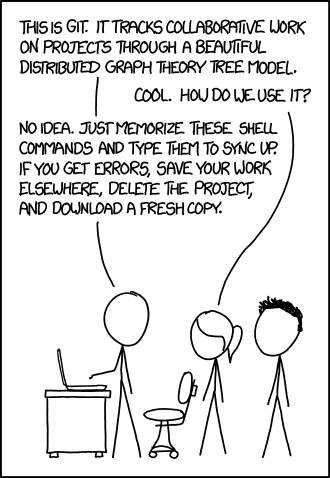
\includegraphics[width=0.4\linewidth]{Im/git_xkcd.png}
	\end{center}
\end{frame}

\begin{frame}[fragile]{Comment ça marche ?}
	\framesubtitle{Comment ça marche ?}
	
	%spongebob meme about magic 
	git est magic!
	\begin{center}
		
\includegraphics[width=0.4\linewidth]{Im/its-a-kind-of-magic.jpg}
	\end{center}

	il peut faire tout ce que vous voulez, mais il faut savoir comment lui demander

\end{frame}

\begin{frame}{Quels sont les avantages ?}
	% \begin{column}{0.5\linewidth}
		en quoi git est-il mieux que les autres méthodes ?
		% \begin{column}{0.5\linewidth}
			\begin{itemize}
				\item <1-> Historique des modifications
				\item <2-> Sauvegarde
				\item <3-> Commentaires
				\item <4-> Automatisation
			\end{itemize}
		% \end{column}
		% \begin{column}{0.5\linewidth}	
			% \begin{overprint}
			% 	% on the first slide we will show the 2 screenshots of the code and the code modification and onder a 3rd image with the change in the code
			% 	\onslide<1>{
			% 		\begin{subcaptiongroup}
			% 			\begin{subfigure}{0.3\linewidth}
			% 				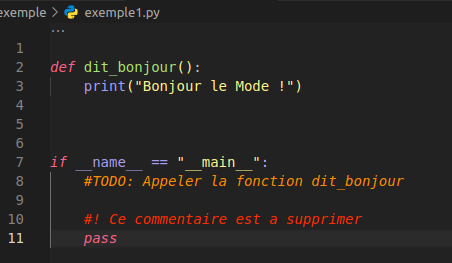
\includegraphics[width=\linewidth]{Im/exemple/pre_modif.png}
			% 				\caption{Code original}
			% 			\end{subfigure}
			% 			\begin{subfigure}{0.3\linewidth}
			% 				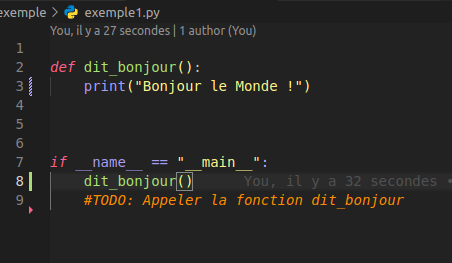
\includegraphics[width=\linewidth]{Im/exemple/post_modif.png}
			% 				\caption{Différence}
			% 			\end{subfigure}
			% 			\begin{subfigure}{0.3\linewidth}
			% 				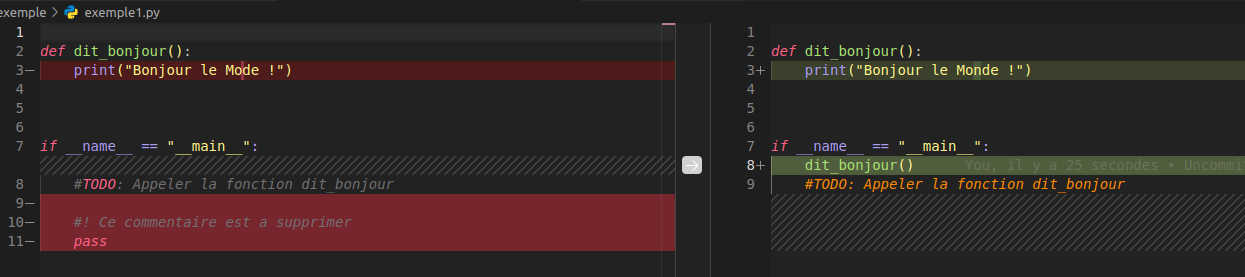
\includegraphics[width=\linewidth]{Im/exemple/modif_visualisation.png}
			% 				\caption{Code modifié}
			% 			\end{subfigure}
			% 		\end{subcaptiongroup}
			% 		}
			% \end{overprint}
		% \end{column}
	% \end{column}
\end{frame}
	
	


\begin{frame}[fragile]{Comment utilser ?}
	les commandes de base:
	\begin{itemize}
		\item git init
		\item git add
		\item git commit
	\end{itemize}

	les commandes un peu plus avancées (surtout utile en collaboration)
	\begin{itemize}
		\item git branch
		\item git checkout et git switch
		\item git merge
	\end{itemize}

	% bloc pour dire que on ne va que voir les commande sur la ligne de commande
	\begin{alertblock}{Note}
		Nous ne verrons que les commandes en ligne de commande, mais il existe des interfaces graphiques pour git (voir \ref{sec:aller-plus-loin})
	\end{alertblock}
\end{frame}


\begin{frame}[fragile]{les commandes de base}
	\begin{itemize}
		\item<1-4> git init
		\item <2-4> git status
		\item <3-4> git add
		\item <4-4> git commit
	\end{itemize}

	\begin{onlyenv}<1>
		\begin{block}{git init}
			\texttt{git init} permet de créer un nouveau dépôt git dans le répertoire courant sous la forme d'un dossier caché \texttt{.git}
		\end{block}

		\begin{block}{note}
			\texttt{.git} n'as pas besoin d'être modifié directement, il est géré par git lui-même. mais si vous voulez automatiser des tâches, vous pouvez ajouter des scripts dans le dossier \texttt{.git/hooks}
		\end{block}

		commande à taper: \lstinline|git init|
	\end{onlyenv}

	\begin{onlyenv}<2>
		\begin{block}{git status}
			\texttt{git status} permet de voir l'état de votre dépôt git, c'est-à-dire les fichiers qui ont été modifiés, ajoutés, supprimés, \dots
		\end{block}

		commande à taper: \lstinline|git status|
	\end{onlyenv}

	\begin{onlyenv}<3>
		\begin{block}{git add}
			\texttt{git add} permet d'ajouter des fichiers à l'index de git, c'est-à-dire de dire à git que vous voulez suivre les modifications de ce fichier et % add color to the text
			quand vous ferez un commit, 
			\color{red}
			Uniquement
			\color{black}
			les modifications de ces fichiers seront prises en compte.
		\end{block}

		commande à taper: \lstinline|git add <fichier>| \\
		
		\texttt{<fichier>}: peut être un fichier ou un dossier
	\end{onlyenv}

	\begin{onlyenv}<4>
		\begin{block}{git commit}
			\texttt{git commit} permet de sauvegarder les modifications de vos fichiers dans le dépôt git. il est important de mettre un message clair et concis pour expliquer les modifications apportées.
		\end{block} 

		commande à taper: \lstinline|git commit -m "message"| \\
		le -m est obligatoire et le message doit être entre guillemets
	\end{onlyenv}
\end{frame}
\begin{frame}[fragile]{les commandes de base}
	Bravo vous avez fait votre premier commit !
	\pause
	\begin{center}
		
\includegraphics[width=0.5\linewidth]{Im/question-mark.png}
	\end{center}
	bon maintenant comment voir ce que vous avez fait ?
\end{frame}

\begin{frame}[fragile]{les commandes de base}
	% insert 2 images side by side with the git log and the git tree
	\begin{columns}
		\begin{column}{0.5\linewidth}
			\lstinline|git log| \\
			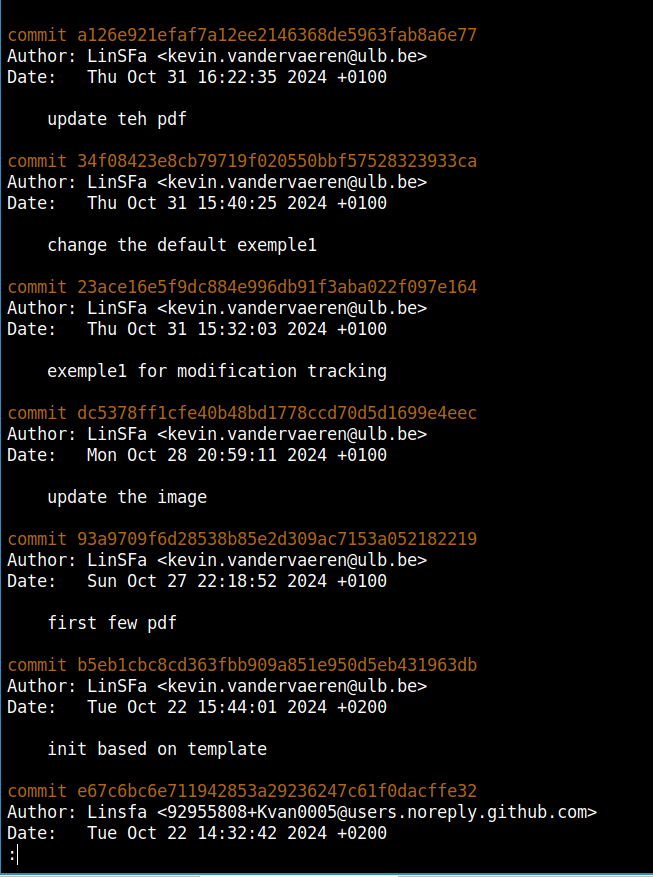
\includegraphics[width=\linewidth]{Im/exemple/terminal_log.png}
		\end{column}
		\begin{column}{0.5\linewidth}
			git graph sur vscode\\
			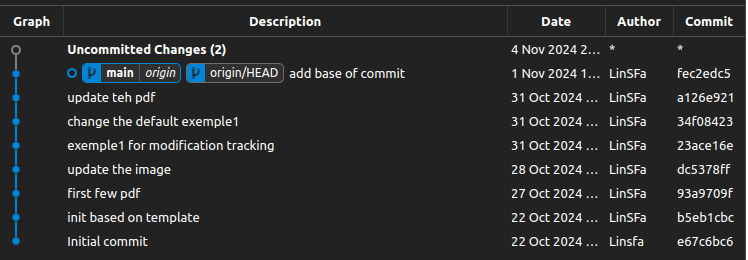
\includegraphics[width=\linewidth]{Im/exemple/vs_log_tree.png}
		\end{column}
	\end{columns}
\end{frame}

\begin{frame}[fragile]{Introduction a GitHub}
	Avant de continuer, avez-vous des questions ?
	\pause
	\vspace{2cm}
	Avant les commande un peu plus avancées, nous allons voir comment utiliser GitHub
\end{frame}



\begin{frame}[fragile]{Introduction à GitHub}
	\begin{itemize}
		\item En quoi est-ce différent de Git ?
		\item Comment l'utiliser ?
		\item avantages et inconvénients
	\end{itemize}
\end{frame}

\begin{frame}[fragile]{En quoi est-ce différent de Git ?}
	simple analogie:
	\begin{center}
		
\includegraphics[width=0.70\linewidth]{Im/git_porn.png}
	\end{center}
\end{frame}
\begin{frame}[fragile]{En quoi est-ce différent de Git ?}
	Si git est un livre, alors GitHub est une bibliothèque où vous pouvez stocker vos livres et les partager avec d'autres personnes.
	\vspace{2cm}
	Git sont vous données, Git est un cloud pour les stocker et les partager
\end{frame}

\begin{frame}[fragile]{En quoi est-ce différent de Git ?}
	
	\begin{center}
		
\includegraphics[width=0.3\textwidth]{Im/Git-logo.png} 
		\hspace{1cm}
		\textbf{\LARGE VS}
		\hspace{1cm}
		\includegraphics[width=0.3\textwidth]{Im/github-logo.png}
	\end{center}
	\begin{table}[h!]
		\centering
		\begin{tabular}{|c|c|}
			\hline
			\textbf{Git} & \textbf{GitHub} \\
			\hline
			\hline
			programme & service \\
			\hline
			\begin{tabular}[c]{@{}c@{}}gestion de version \\ décentralisé\end{tabular} & \begin{tabular}[c]{@{}c@{}}plateforme de \\ collaboration\end{tabular} \\
			\hline
			local & en ligne \\
			\hline
			open source & propriétaire (Microsoft) \\
			\hline
		\end{tabular}
	\end{table}
\end{frame}
\begin{frame}[fragile]{alternatives à GitHub}
	% add a list of multiple image of the logo of different git hosting service
	\begin{center}
		
\includegraphics[width=0.45\linewidth]{Im/gitea-logo.png}
		
\includegraphics[width=0.45\linewidth]{Im/gitlab-logo.png}
	\end{center}
	\begin{center}		
		
\includegraphics[width=0.3\linewidth]{Im/bitbucket-logo.png}
	\end{center}

	et bien d'autres...

\end{frame}

\begin{frame}[fragile]{comment l'utiliser ?}
	\begin{itemize}
		\item créer un compte
		\item clee d'accès ?
		\item premier dépôt (aka repo)
	\end{itemize}
\end{frame}

\begin{frame}[fragile]{créer un compte}
	avez vous vraiment besoin d'une explication ?

	\begin{blueblock}{conseil}
		apres avoir créé votre compte, vous pouvez utilser le GitHub sudent pack pour avoir des avantages supplémentaires 
	\end{blueblock}
\end{frame}

\begin{frame}[fragile]{clée d'accès}
	\begin{itemize}
		\item<1-> pourquoi ?
		\item<2-> comment ?
	\end{itemize}
	\begin{onlyenv}<1>
		\begin{block}{pourquoi ?}
			utiliser par github pour vous identifier, elle vous permet de vous authentifier quand vous fait des actions sur votre compte (clone, push, pull, \dots)
		\end{block}
	\end{onlyenv}
	\begin{onlyenv}<2>
		\begin{block}{comment ?}
			suivant les étapes suivantes:
			\begin{itemize}
				\item aller dans les paramètres de votre compte se trouvant en haut à droite
				\item settings de developer (ou alors SSH and GPG key mais c'est hores sujet)
				\item clée d'accès personnel (personal access token) 
				\item Tokens (classique)
				\item générer un nouveau token et donner toutes les permissions (par simplicité)
				\item \textbf{copier le token et le garder en lieu sûr}
			\end{itemize}
		\end{block}
	\end{onlyenv}
\end{frame}

\begin{frame}[fragile]{premier dépôt}
	crée un nouveau dépôt:
	\begin{itemize}
		\item aller sur la page d'accueil de votre compte
		\item cliquer sur le bouton "new"
		\item donner un nom à votre dépôt
		\item ajouter une description
		\item choisir si vous voulez un dépôt public ou privé
		\item cliquer sur "create repository"
	\end{itemize}
	simple non ?
\end{frame}

\begin{frame}[fragile]{comment l'utiliser ?}
	comment iteragir avec un dépôt GitHub ?
	\begin{itemize}
		\item git clone
		\item git push
		\item git pull
	\end{itemize}
\end{frame}


\begin{frame}[fragile]{les commandes un peu plus avancées}
	\begin{itemize}
		\item git branch
		\item git checkout et git switch
		\item git merge
	\end{itemize}
\end{frame}

\begin{frame}[fragile]{les commandes un peu plus avancées}
	\begin{itemize}
		\item<1-3> git branch
		\item <2-3> git checkout et git switch
		\item <3-3> git merge
	\end{itemize}

	\begin{onlyenv}<1>
		\begin{block}{git branch}
			\texttt{git branch} permet de créer une nouvelle branche dans votre dépôt git. une branche est une copie de votre code à un moment donné, vous pouvez travailler sur cette branche sans affecter le code de la branche principale (master).
		\end{block}

		commande à taper: \lstinline|git branch <nom_branche>|
	\end{onlyenv}

	\begin{onlyenv}<2>
		\begin{block}{git checkout et git switch}
			\texttt{git checkout} et \texttt{git switch} permettent de changer de branche. \texttt{git checkout} est la commande historique, mais \texttt{git switch} est plus intuitive.
		\end{block}

		commande à taper: \lstinline|git checkout <nom_branche>| ou \lstinline|git switch <nom_branche>|
	\end{onlyenv}

	\begin{onlyenv}<3>
		\begin{block}{git merge}
			\texttt{git merge} permet de fusionner une branche avec une autre. il est important de faire attention à ce que vous fusionnez, car si vous avez des modifications sur les mêmes fichiers, git ne saura pas quoi faire.
		\end{block}

		commande à taper: \lstinline|git merge <nom_branche>|
	\end{onlyenv}
\end{frame}

\begin{frame}[fragile]{commandes un peu plus avancées}
	\begin{center}
		
\includegraphics[width=0.7\linewidth]{Im/merge_outcome.jpg}
	\end{center}
\end{frame}

\begin{frame}[fragile]{commandes un peu plus avancées}
	comment résoudre un conflit ?
	\begin{blueblock}{résoudre un conflit}
		\begin{itemize}
			\item ouvrir le fichier en conflit
			\item chercher les balises de conflit
			\item résoudre le conflit
			\item ajouter les fichiers modifiés
			\item faire un commit
		\end{itemize}
	\end{blueblock}
\end{frame}


\begin{frame}[fragile]{exercices pratiques}
	\begin{itemize}
		\item exercice 1: créer un dépôt git
		\item exercice 2: faire un commit
		\item exercice 3: créer une branche
		\item exercice 4: fusionner une branche
		\item exercice 5: résoudre un conflit 
	\end{itemize}
\end{frame}

\end{document}
